% HEADER Section
% Define formal of the paper
\documentclass[sigconf, natbib=false]{acmart}
\setcopyright{none} % Remove the 
\settopmatter{printacmref=false} % Removes citation information below abstract
\renewcommand\footnotetextcopyrightpermission[1]{} % removes footnote with conference information in first column
\pagestyle{plain} % removes running headers
\setlength{\marginparwidth}{2cm}
\usepackage{outlines} % item and sub items 
\usepackage{pifont} %provides addition symbols


%% Include packages 
\usepackage[style=ACM-Reference-Format,backend=bibtex,sorting=none]{biblatex}
\addbibresource{ref.bib}
\usepackage{lipsum}% for dummy text
\usepackage[parfill]{parskip} % create space between paragraph
\fancyfoot{}
\usepackage{booktabs} % For formal tables
\usepackage{subcaption}

% package for drawing flowchart 
\usetikzlibrary{shapes.geometric, arrows}
\usepackage{caption}  

% package for to do 
\usepackage{xcolor}
\newcommand\mytodo[1]{\textcolor{red}{#1}}
\usepackage{todonotes}

% packages for pseudo code 
% \usepackage{algorithm} 
% \usepackage[noend]{algpseudocode}
% \usepackage{algpseudocode}
\usepackage{algcompatible}
\usepackage[noend, ruled,lined]{algorithm2e}

% Drawing figure with tikz package
\usepackage{tikz}
\usetikzlibrary{positioning, shapes}



%table 
\usepackage{multirow}
\usepackage{graphicx}

\newcommand\MyBox[2]{
  \fbox{\lower0.75cm
    \vbox to 1.7cm{\vfil
      \hbox to 1.7cm{\hfil\parbox{1.4cm}{#1\\#2}\hfil}
      \vfil}%
  }%
}

% Paraphase, grammer 



%% Author Information 
\title{A Data-Driven Machine Learning Approach to Detect Suspicious Companies}
\author{Asif Anwar (2660561)}
\affiliation{%
  \institution{Vrije Universiteit}
  \streetaddress{ De Boelelaan 1105}
  \city{Amsterdam} 
  \country{The Netherlands} 
  \postcode{1081 HV}
  }
\email{a.anwar@student.vu.nl}


% Main report 

\begin{document}



\begin{titlepage}
    \begin{center}
    \vspace{0.8cm}
        
\includegraphics[width=0.4\textwidth]{figures/vua.pdf}
        \vspace*{1cm}
        
        \Huge
        \textbf{A Data-Driven Machine Learning Approach to Detect Suspicious Companies}
        % \textbf{Eagle Eye: Trade Fraud Detection Using Machine Learning Techniques}
        
        \vspace{0.5cm}
        \LARGE
        Master Thesis \\
        
        
        \vspace{2.5cm}
        \large
        Author: \\
        \vspace{0.25cm}
        \Large
        Name: \textbf{Asif Anwar}\\
        \vspace{0.25cm}
        \large
        Id: AAR216\\
        \vspace{0.25cm}
        Email: A.Anwar@student.vu.nl\\
        
        \vspace{1.5cm}
        \large
        supervisor: \\
        \vspace{0.25cm}
        \Large
        \textbf{Dr. Charlotte GerritsenDaily}
        

        
        \vfill 
        
        \today \\
        \vspace{0.5cm}
        Submitted in partial fulfillment of the requirements for\\ 
        the degree of Master of Science in Artificial Intelligence. 
        
        \vspace{1cm}
        
   
        
        \vspace{2.5cm}
        
        
    \end{center}
\end{titlepage}

\newpage
    \thispagestyle{empty}
    \tableofcontents
\newpage

\begin{abstract}
    Trade credit fraud is a major concern for suppliers and insurance companies. An accurate and effective classification method can reduce potential financial loss, as well as reduce massive operational cost for the organisations. However due to large amount of unstructured data and high class imbalance, fraud classification is a enormously challenging task. The goal of this paper to find the suitable machine learning model to identify suspicious companies. A data driven approach has been applied to extract features and generate the required dataset. Then different machine learning techniques have been used to handle imbalance classes and build models. based on different performance matrices like ROC, AUC, confusion metrics, mean recall  are used to find the best models and Threshold limits to fine tune to model. \\
    results:\\
    Results of random forest classifier are more accurate than other machine learning algorithm.
    
\end{abstract}
\keywords{Fraud Detection, Machine Learning, SOMTEC, Data Mining}

\maketitle
\pagestyle{plain}
\balance

% Include Sections 
\section{Introduction} \label{sec: Intro}
% This section includes some motivations behind the work, explicitly or implicitly highlights the research question , provides a high-level explanation of the solution, and describes the contributions.

% establish the context, background and/or importance of the topic
In the current global economy, the financial fraud has become a crucial issue especially for the trade sector. In recent times, the number of fraud cases have increased drastically which effected both financial institutions and their clients significantly. From a survey in 2020 on economic crime and fraud by Price Waterhouse Coopers, its been reported that more than 42 billion USD of financial losses happened in past 24 months~\cite{PwC.Crime.Survey}. On an average companies reportedly experienced 6 fraud cases during this period. Thirty five percent of fraud cases are marked as Customer fraud~\cite{PwC.Crime.Survey}.   

In current trend, more and more, companies outsource non-core activities to third party companies to reduce operational costs. But these third party-party business partners can be fraught with risk. One in five respondents from the PwC survey~\cite{PwC.Crime.Survey} cited vendors/suppliers as the source of their most disruptive external fraud. On the other hand, suppliers are also in high risk of fraud cases from their buyers. Due to this detecting suspicious companies (buyers and suppliers) plays an important role to reduce financial losses for the trade insurance companies and theirs customers.


% brief synopsis of the relevant literature
Fraud or extortion is a par of internal threats for any business. Manufacturers and service providers may face financial losses from fraudulent buyers. According to Association of Certified Fraud Examiners (ACFE), the definition of fraud is "the use of one\’s occupation for personal enrichment through the misuse or deliberate
misapplication of the resources or assets of the employing organization"~\cite{kassem_2014}. To term fraud that is imposes to manufactures and service provider it can be redefined as the personal gain of the buyers by misuse or deliberate misapplication of the products and services of the supplying organization and their respective insurance companies.

% Indicate an issue, problem or controversy in the field of study

A classical approach to prevent such fraudulent cases is done by traditional method of using human resources like internal and external auditors~\cite{kassem_2014}, and business team. Each team has their own process of monitoring external partners and buyers by analyzing transaction patterns, financial overview, historical behaviour to identify suspicious companies.  Based on the organizational capabilities, these team uses different internal and external resources like archival system, reports and news source.


Historically, organizations and financial institutions are using different technological solutions and operational process to detect suspicious companies. In the technological solutions different software are used to verify names, previous history and financial status of the buyers. On the other hand, as part of operational process during the customer on-boarding the Know Your Customer (KYC) process are used to identify anomaly in the customer profile. However, the major problems for these existing solution to detect suspicious companies are complex, time consuming, costly,and cognitively challenging labor intensive task.


However, in recent past with the advancement of artificial intelligence and data mining techniques, different machine leaning solutions are developed to find anomalies, credit card fraud, etc.~\cite{RB2021, KIRKOS2007995}. Considering the complexity of the tasks the continuous improvement of the systems are going on. The incremental success of these solutions are showing a great promises to reduce operations time and cost for the organizations and financial institutions.

Most studies in the field of suspicious activity classification for economical sector are done on Credit Card fraud detection. The recent number of individual and organized criminals the number of credit card has increased significantly ~\cite{RB2021}. Although lots of research has been carried out on detecting anomalies in financial crime, we can see that most of the researches for identifying suspicious financial crime activity are focused on detecting credit card fraud. However, as mentioned earlier, in the survey from PwC we have seen that third party business crime and fraud imposes high risk and have huge financial impact on the economy.
% listing the reasarch question or hypotheses


This paper will focus on using a data-driven approach using machine learning techniques to detect suspicious companies to prevent financial losses for the organizations and respective financial institutions.  The major objective of this study is to use data mining technique to extract features from unstructured data, and apply ensemble learning and neural network to identify the pattern on the features to detect suspicious companies.

% provide synopsis of the research methols



Data extracted is a useful method to gather data for analysing and prediction tasks. Data driven is a method base on the history data to build more hyper-parameters to compensate the un-measurable features within the measurable data \cite{SMARRA20181252}. some extending nonlinear features to build the prediction function. In classification and prediction problem, it is essential to discover the pattern of the data and provide us some insights to take some actions according to the prediction results. Random Forest algorithm and Neural Networks are been used in handling this problem and shown effective~\cite{10.1145/3414274.3414278, RB2021}. However it is extremely hard to identify the target information from institutions data based on pattern. The propose of the paper is to find a suitable classifier and its application to find fraudulent cases based on assembly learning and machine learning .





% Significance of value of the study

% Define the topic or key term

% Overview of teh report stucture

% State the purpose of the essay / write

% Provide an overview of the coverage





\section{Background} \label{sec: background}
% This section provides the necessary context to help the reader understand the remainder of the thesis.

% Why this report is generated

In the section~\ref{sec: Intro}, its been highlighted how fraud can impact the business and overall economy. As per the PwC survey on crime and fraud~\caption{1} we can see that companies who invested money on fraud prevention had to pay 16\% less fine and\/ or penalties than who didn't~, as shown in figure~\ref{fig:fraud_preven}. Hence to protect financial and reputation losses, the companies have to invest money and effort. However the existing process is costly and human intensive. The paper focus on how a machine leaning based system can help the companies to reduce the overall operational cost and save financial losses.

The aim of this paper is to perform a data driven approach to extract relevant data to build machine learning classification model to detect specious company for a leading trade credit insurance provider. The trade credit insurance provides protection to the business (customer of the insurance company) in the event their buyers fail to pay for the products or services. Considering the raise of fraudulence business in recent past, the insurance provider has to monitor each buyers extensively before approving any insurance policy. Considering the number of number of policies are so high, a machine learning based recommended system was implemented for UK market to detect suspicious companies. Since the implementation of the system the solution saved around 1M pounds. Due to the success of the UK model, the organization decided to implement similar recommendation ending in other market.

\begin{figure}[htp]
    \centering
    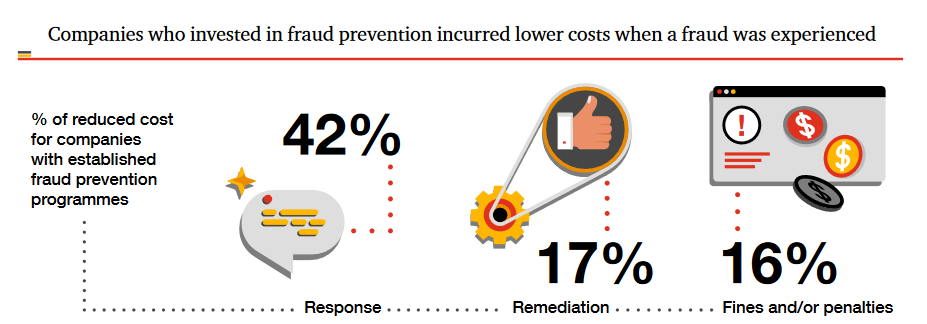
\includegraphics[width=\linewidth]{figures/prevent_fraud.PNG}
    \caption{Investment on Fraud Prevention. Source: PwC 2020 Fraud survey~\cite{PwC.Crime.Survey} }
    \label{fig:fraud_preven}
\end{figure}

For this paper, the a model focuses on identifying suspicious companies for Italian Market. Each country is fundamentally different in terms of trade credit policy. Hence, each country has its own internal process and method to identify the suspicious cases. To build the recommendation model below data driven machine learning strategies are used.

\mytodo{update terms: buyers, client and provider}

\subsection{Trade Credit Insurance}\label{subsec:trade-credit-insurance}
In business world trade credit is a regular practice done by manufactures, suppliers, and service providers to protect their financial interest from any types of risks.\mytodo{find the total yearly trade credit amount}. Companies sales their products and goods on credit to their buyers. Generally this is a continues process as back to back trade deals and payment happens between the suppliers and buyers. However, the amount of trade credit is very high, hence suppliers like to protect their interest by taking credit polices from financial institutions  \mytodo{cite what is trade credit}.

For financial institutions (credit insurance provider) ensures financial support to the supplier (client) in event of any mishaps. Trade credit is a risky business, hence before providing any insurance, financial institutions verifies both both supplier, sales, global economic conditions, external factors. As mentioned in section~\ref{sec: Intro}, due to the increased number of fraud cases, insurance providers have to also monitor fraudulent cases. Below are the types of fraud happens in the trade credit sector.

\begin{itemize}
    \item \textbf{Buyers Fraud:} When the buyers of the goods and products get benefited by not paying the dues to the suppliers.
    \item \textbf{Client Fraud:} When suppliers, the clients of the insurance company try to economic gain by doing insurance fraud.
    \item \textbf{Joint Fraud:} When the suppliers and buyers cooperate together to conduct insurance fraud get economic gain.
    \item \textbf{Internal Fraud:} When internal parties from the insurance company colludes with the client and conduct an insurance fraud.
\end{itemize}

In this study we will mainly focus on finding the suspicious buyers to prevent economic mishaps to protect the suppliers and the insurance companies from financial loss.


\subsection{Monitor Credit Policy}\label{subsec:monitor-credit-policy}

\subsubsection{Issuing Trade Insurance}\hspace*{\fill} \\
The trade insurance providers go through a sequence of steps to approve or issue a credit policy to their clients. In the the figure~\ref{fig:trade_credit}, the process of trade credit issuance is shown. First the client (supplier) requests for a credit policy to the trade credit insurance provider after they get a formal purchase request from their buyer. Based on the client's requests, the credit undertaking team of the insurance provider verifies the client, its buyer, the amount and other respective details of the transactions. If the credit undertaking team find the request as legitimate then they inform the internal operation team to issue a policy to the client. On a event the buyer fails to pay back for the goods, the supplier (client) applies for insurance claim from the service provider. After a thorough investigator the insurance provider pays the money to the supplier and tries to collect the money from the buyers to reduce its operational loss.

\begin{figure}[htp]
    \centering
    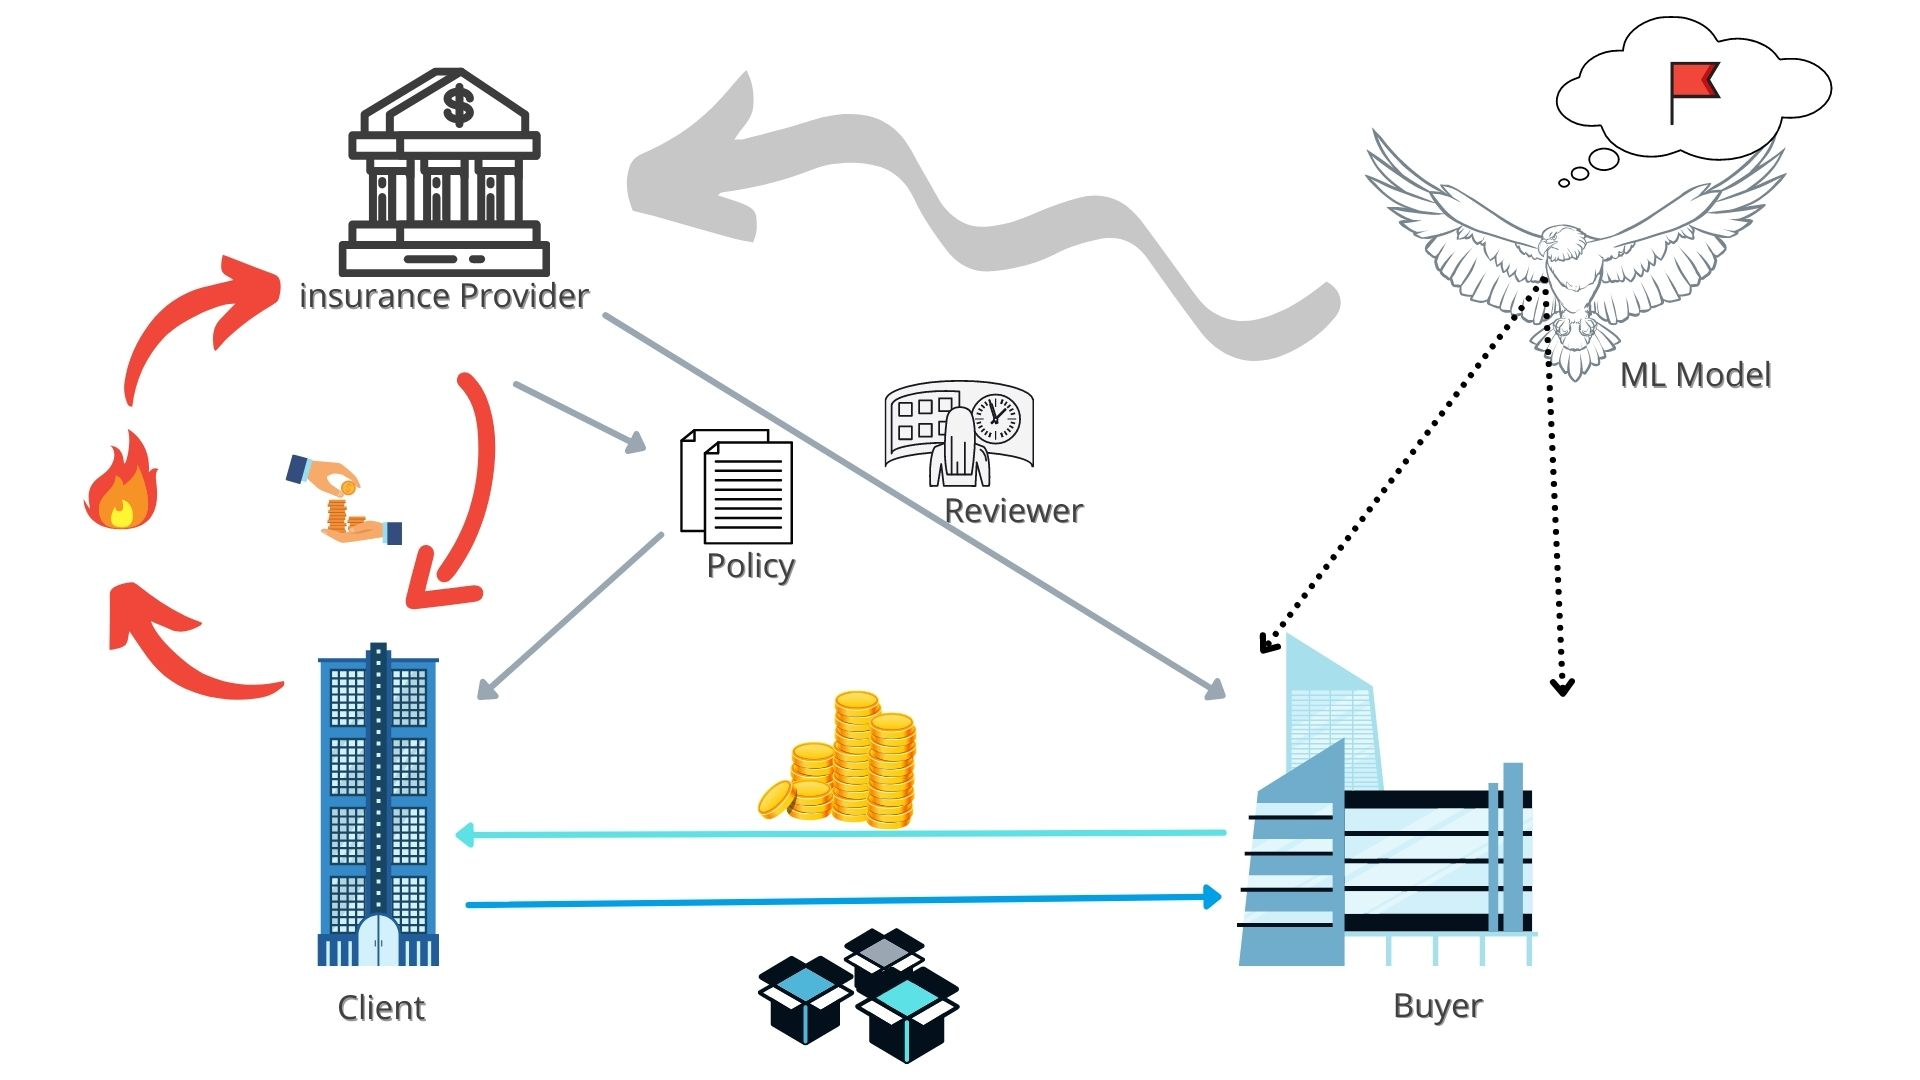
\includegraphics[width=\linewidth]{figures/monitor_buyers.jpg}
    \caption{Trade credit issuing process}
    \label{fig:trade_credit}
\end{figure}


As mentioned earlier in this chapter, there are four different types of fraud can take place in trade credit insurance sector. As the report only focuses on the buyers fraud, the existing monitoring process and proposed monitoring process are mentioned below to identify suspicious buyers.
\subsubsection{Traditional Approach}\hspace*{\fill} \\

The traditional way of identifying suspecious buyers are done by reviews from the credit undertaking team of the insurance service provider. As mentioend in Section~\ref{sec: Intro} below tools and techniques are currently use by the team.
\begin{itemize}
    \item{Internal System:} The reviews looks for suspecious patterns on the comapny reports and different system inicators to identify any suspecious companies.
    \item{External System:} The reviews also go through some external links provided by global ALM and regulatory systems to avoid any existing risks.
    \item{Overall Review:} Beside the above system, there are mutiple layes of monitoring done by different reviews to reduce operational errors.
\end{itemize}

\subsubsection{Machine learning base Approach}\hspace*{\fill} \\

In the proposed data-driven machine learning technique, a suitable model will be developed based on the data extracted from different system by taking input from the experts. Everyday the latest policy requests will be fed to the model so that it can predict the highly specious companies. The highlighted companies will be then shared with the credit undertaking team to expedite their reviewing / monitoring process. Based on the outcome and feedback of the reviewr, the model will be continuerly updated to improve its performance.




\section{Related Work}\label{sec:related-work}

Some of the related study made by various researchers is described in this section. The researches varies from different types of machine learning techniques to various methods for data mining and prepossessing. The main recherche topics are focused on finding fraudulent transaction using machine learning methods. 


Asha RB and Suresh Kumar KR proposed a method to detect the fraud in credit card transactions that is based on deep learning \cite{GoodBengCour16} in the paper credit card fraud detection using artificial neural network \cite{RB2021}. Frauds in credit card transactions are most common and frequent issue. In the paper the researcher usages support vector machine (SVM) \cite{Cristianini2008}, k-nearest neighbour (KNN) \cite{Mucherino2009} and artificial neural network (ANN). The paper conclude that artificial neural network (ANN) gives accuracy of 0.99 with precision of 0.81 and recall of 0.76.


Class imbalance is a major challenge for classifying normal and fraudulent cases. In the paper "Deep Over-sampling Framework for Classifying Imbalanced Data" \cite{ando2017deep} Shin Ando and Chun Yuan Huang has proposed a framework which extending the synthetic over-sampling method to the deep feature space acquired by a convolutional neural network (CNN) \cite{Yamashita2018}.Deep Over-sampling uses the overloaded instances to supplement the minority classes.  

In the paper "Data Mining techniques for the detection of fraudulent financial statements" \cite{KIRKOS2007995}, Efstathios Kirkos, Charalambos Spathis, and Yannis Manolopoulos explores the effectiveness of Data Mining (DM) classification techniques in detecting firms that issue fraudulent financial statements. Data Mining proposes several classification methods
derived from the fields of statistics and artificial intelligence. As per the research three methods, which enjoy a good reputation for their classification capabilities

Kamat Nath Mishra and Subhash Chandra proposed a k-fold machine learning techniques for fraud prediction in smart societies \cite{Mishra2021}. In their paper on fraud detection they have classified the types of credit card fraud types. They proposed a logistic regression based solution. The implementation of their methodology is then further analysed using machine learning tools like ROC curve \cite{FAWCETT2006861}, confusion matrix, mean-recall score value and precision recall curve. 

In the paper "Imbalanced classification Problem Using Data-driven and Random Frost Method" \cite{10.1145/3414274.3414278} the researcher Wan Wang, Xinglu Liu and Victor Chan proposed a classification method for imbalanced dataset using data driven technique and random forest. The research is done over three open-source dataset. The result shows that random forest applied with data driven approach improved the prediction accuracy. The AUC values also perform well stable and even increased. The researcher augured that they used imbalanced dataset which represent real world data. So in theory their approach should perform reasonably in real world scenarios. 

Important insights for selecting machine learning algorithm for skewed dataset has been discussed in the paper "The relationship between precision-recall and ROC curves" \cite{davis06}. As per the researcher Jass Davis and Mark Goadrich, ROC space and PR space have a deep connection. When a curve dominate in ROC space it also dominates in PR space. They also shared that a model which optimised the area under the ROC curve are not guaranteed to optimised the area under the PR curve. This study can be really handy for our use case of fraud detection. 

In The literature review named "Fraud detection using the fraud traiangle theory and data myning techniques" \cite{computers10100121} the researchers highlighted the complexity on predicting Fraud. They explained the human behavioural aspect of fraudulent activity and how traditionally detection was performed by auditors and manual technologies. The researcher mentioned in the paper, in recent past how several works related to fraud detection using
machine learning techniques were identified without the evidence that they incorporated the fraud triangle as a method for more efficient analysis. \label{sec: related work}
\section{Overview}\label{sec: Overview}
% This section provides a high-level outline of the proposed system or solution. It typically illustrates the system architecture or the interactions between the different solution components (via a “boxes-and-arrows” diagram) from a user’s perspective.


A joint data-driven technique and machine learning algorithms approach are used in this work for this classification task. Before the classification step, the number of new features are generated or engineered from the internal company data. the insight from the experts are considered first, then from the historical reports, the data-driven method was used to prepare a dataset to train the desired model. Based on statistical correlation the important features are selected as final features to train various Ensemble models and artificial neural networks are used to get the best outcome\ref{fig:class distribution}. 

The first step of the data-driven approach is to apply the theory of change. As per the theory of change, we can find the road map for how to get company information which is most useful. This method also helps to find how to archive long time goals along with an indicator for improving and tracking progress. Then it is important to get in touch with internal experts to understand what sort of data they are using for daily tasks.

Generally, the classifiers perform quite weak due to missing values and an imbalance dataset for real-life scenarios. One of the major reasons for the missing data is the collected data does not contain enough information, because of the statistical error or some missing values. To obtain more hidden information, a data-driven method generally is a good choice. In the data-driven approach, hidden features can be found based on feedback from expert

Data-driven decision making means getting the right data to the right model at the right time to improve the model for problem-solving. This approach can help the organisation to identify and apply recent trends in data to apply it for finding solutions.

\subsection{Proposed architecture}\label{subsec:propsed-architech}
In the figure~\ref{fig:flow} the proposed architecture for the end to end solutions is given. In this overall design, the model training and evolution will be done by using historical company data. A regular data feed will be provided in the model for doing the recommendation or classification. Based on users feedback the system will be improved in time. 

\begin{figure}[ht]
    \centering
    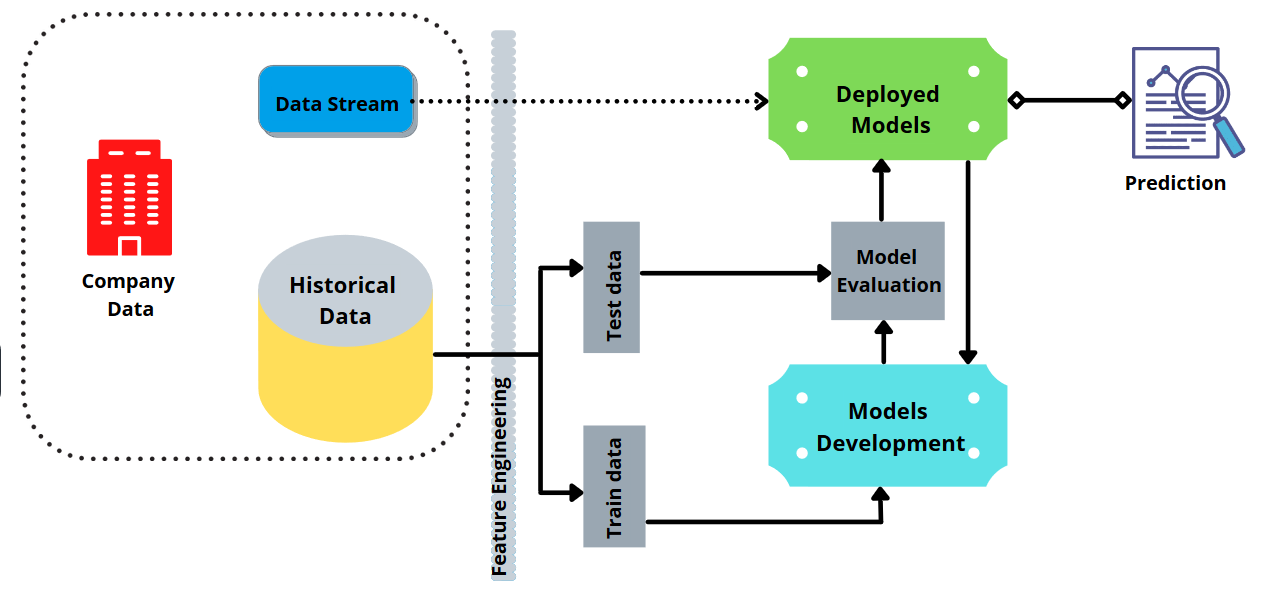
\includegraphics[width=\linewidth]{figures/overall_design.PNG}
    \caption{Overall Design}
    \label{fig:flow}
\end{figure}

The rest of this section will cover different techniques and methods, which are necessary to build a suitable solution for the given problem. 



\subsection{Imbalance Class Problem}\label{subsec:imbalance-class-problem}
Training classification model using imbalance data set generally leads to bias to predict one sample from another. Considering the number of fraudulent or suspicious companies are so less, the training data set for fraud detection is highly imbalanced. Before training the classifier, the data set can be fixed by using the below sampling methods.  

\subsubsection{Under-sampling:}\hspace*{\fill} \\
Under-sampling is one of the common and basic methods of sampling to reduce class biases \cite{10.1145/3055635.3056643}. In this method, a selective number of (generally equal number of smaller class data) samples are taken from large classes. The samples are randomly taken and the number of instances is based on minority class. This method provides a smaller dataset than the actual one as the number of instances for the majority class reduces dramatically. 

\subsubsection{Over-sampling}\hspace*{\fill} \\
For the over-sampling method, more samples are taken from the minority class so that the main dataset becomes balanced. Even though the random sampling method is used for taking samples, but due to class imbalance, we can see that number of repeated instances are copied from the minority class to prepare the dataset. This method provides a larger dataset as the number of instances for minority classes increases. 

\subsubsection{SMOTE}\hspace*{\fill} \\
SMOTE is a synthetic oversampling method \cite{2002}. SMOTE drastically improve the performance of classifying minatory class by creating synthetic samples. Generally, the synthetic samples are randomly generated by randomly selected minority class samples with interpolation between the neighbours of the selected sample. SMOTE facilitate a balanced dataset with related minority class samples to learn from, which allows the models to decision border regions,  leading to coverage of the minority class.

\subsubsection{Combined Sampling}\hspace*{\fill} \\
In the combined sampling method, two or more samplings methods are used in the same data set \cite{10.1145/3055635.3056643}. Under and oversampling is a common approach. In this method, the under-sampling of the majority class and oversampling of the minority class is done to prepare the Dataset. Another suitable method is to under-sample the majority class and synthetic sampling the minority class. 

% Source from paper 31
\subsection{Model Selection}\label{subsec:model-selection}

\subsection{Ensemble learning}\label{subsec:ensemble-learning}\hspace*{\fill} \\
As they use a collection of results to make a final decision, they are referred to as ensemble techniques.


\begin{outline}
 \1 \textbf{Random Forests:} Random forest classified is designed based on decision tree A is a decision tree in classification tree which each node has a  decision based on binary whether  $x_i < \alpha$ or $\alpha$  not for a fixed. The random forests classifiers are a combination of a large number of decision tree algorithms \cite{breiman2001random} ensemble together. Random forest algorithm is designed in such a way that it combines a large number of relatively uncorrelated decision trees \cite{breiman2001random}. The random forest performs better than a single decision tree especially in handling over-fitting and under-fitting for the training set \cite{Mishra2021}. The performance of the random forest algorithm depends on the strength of the individual trees in the forest and the correlation between them. This algorithm also introduces feature randomness by picking up only from a random subset of features which allows it to perform better with classification without over-fitting the training data set. Random forest constructed many individual decision trees at training. Prediction from all trees are pooled to make the final prediction; the mode of the classes for classification.    
 
 \2 Feature Importance: Feature importance is defined based on the probability of finding that particular node by calculating the ratio of samples reaching that node. The higher value gets more importance in feature gets. 
 
 \2 Gini Impurity: Gini impurity is used for classification tasks. $\sum_{i=1}^{C} f_i{(1-f_i)}$, \textbf{$f_i$} is the frequency of label i at a node and \textbf{C} is the number of unique labels. 
 
 \2 Information gain: Information gain is used for splitting the data, by calculating the change in entropy after the dataset split on an node. $Gain(T,X) = Entropy(T) - Entropy(T,X)$, here \textbf{T} is target variable, \textbf{X} is the feature to be split on \textbf{Entropy(T,X)} which is calculated after the data is split on feature~\cite{breiman2001random}.
 
 $$ni_j =w_jC_j - w_{left(j)}C_{left(j)} - w_{right(j)}C_{right(j)}$$
 %\cite https://towardsdatascience.com/the-mathematics-of-decision-trees-random-forest-and-feature-importance-in-scikit-learn-and-spark-f2861df67e3%
 \1 \textbf{XGBoost:} XGBoost is an ensemble method with the main goal of reducing bias and variance. Gradient boosting employs the gradient descent algorithm to minimise loss \cite{Chen:2016:XST:2939672.2939785}. The algorithm forms trees sequentially and each new tree aims to reduce the error of the previous trees (10). The feature weights are readjusted and each new tree learns from its ancestors and the residual error is updated. A strong model is formed by combining successive weak learners which have a high bias to make the final prediction thus reducing both bias and variance.
 
\end{outline}


\subsection{Neural Network}
Artificial neural network is computing system inspired by the biological neural networks~\cite{mcculloch1943logical}. Initially, artificial neural networks were designed based on copying the neural structure of the human brain. Like the human brain, a neural network is composed of artificial neurons which are interconnected based on the system requirements. In each neuron, a non-linearity function was introduced so that the network can learn complex problems. Below are some of the key elements of a standard neural network. 

\tikzset{%
  every neuron/.style={
    circle,
    draw,
    minimum size=0.4cm
  },
  neuron missing/.style={
    draw=none, 
    scale=2,
    text height=0.2cm,
    execute at begin node=\color{black}$\vdots$
  },
}

\begin{figure}[h]
    \centering
        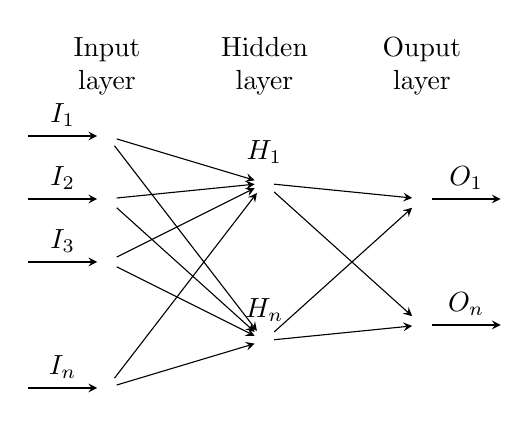
\begin{tikzpicture}[x=1cm, y=0.8cm, >=stealth]
        
            \foreach \m/\l [count=\y] in {1,2,3,missing,4}
              \node [every neuron/.try, neuron \m/.try] (input-\m) at (0,2.5-\y) {};
            
            \foreach \m [count=\y] in {1,missing,2}
              \node [every neuron/.try, neuron \m/.try ] (hidden-\m) at (2,2-\y*1.25) {};
            
            \foreach \m [count=\y] in {1,missing,2}
              \node [every neuron/.try, neuron \m/.try ] (output-\m) at (4,1.5-\y) {};
            
            \foreach \l [count=\i] in {1,2,3,n}
              \draw [<-] (input-\i) -- ++(-1,0)
                node [above, midway] {$I_\l$};
            
            \foreach \l [count=\i] in {1,n}
              \node [above] at (hidden-\i.north) {$H_\l$};
            
            \foreach \l [count=\i] in {1,n}
              \draw [->] (output-\i) -- ++(1,0)
                node [above, midway] {$O_\l$};
            
            \foreach \i in {1,...,4}
              \foreach \j in {1,...,2}
                \draw [->] (input-\i) -- (hidden-\j);
            
            \foreach \i in {1,...,2}
              \foreach \j in {1,...,2}
                \draw [->] (hidden-\i) -- (output-\j);
            
            \foreach \l [count=\x from 0] in {Input, Hidden, Ouput}
              \node [align=center, above] at (\x*2,2) {\l \\ layer};
        
        \end{tikzpicture}
    \caption{Neural Network}
    \label{fig:neural network}
\end{figure}

\begin{outline}
 \1 Activation functions: Activation functions are one of the key elements of the network. These functions create non-linearity between the layers so that the network as a whole can learn to perform complex tasks. 
 
 Sigmoid (eq:~\ref{eq:sigmoid}), Relu (eq:~\ref{eq:Relu}), Softmax are some of the most common activation functions. 
 \begin{equation} \label{eq:sigmoid}
    Sigmoid: \sigma(z) = \frac{1} {1 + e^{-z}}
\end{equation}

\begin{equation} \label{eq:Relu}
    Relu(z) = max(0, z)
\end{equation}

 \1 Loss Functions: The function we want to minimize is the objective function or loss function. For binary classification cross entropy is one of the most common loss function.
    \2 Cross Entropy: In binary classification, where the number of classes \textbf{M} equals 2, Binary Cross-Entropy(BCE) can be calculated as shown in equation \ref{eq:Cross Entropy}. 
    
    \begin{equation} \label{eq:Cross Entropy}
       Cross Entropy Loss: -{(y\log(p) + (1 - y)\log(1 - p))}
    \end{equation}
    
 \1 Optimiser:  The process of minimizing (or maximizing) any mathematical expression is called optimization. Adam optimizer is one the most common optimizer for neural networks. 
    \2 Adam: Adaptive Moment Estimation (Adam) [14] is a method that computes adaptive learning rates for each parameter.  Adam  keeps an exponentially decaying average of gradients. 
 \1 Regularisation: Because the neural network has capabilities to learn complex problem very easily, it tends to over fit the model. To resolve this issue below regularisation methods can be used. 
    \2 Dropout: Dropout is a method to randomly drop neurons during the training so that model doesn't over fit. 
    \2 L1: A regression model that uses L1 regularisation technique is called Lasso Regression. \ref{eq:L1}
    \2 L2: A regression model that uses L2 regularisation technique is called Ridge Regression. \ref{eq:L2}
    
    \begin{equation} \label{eq:L1}
        L1: Loss = Error(Y - \widehat{Y}) + \lambda \sum_1^n |w_i|
    \end{equation}
    
    \begin{equation} \label{eq:L2}
        L2: Loss = Error(Y - \widehat{Y}) +  \lambda \sum_1^n w_i^{2}
    \end{equation}

\end{outline}



\subsection{Tools of Trade}\label{subsec:tools-of-trade}

\subsubsection{Performance Metrics:}\hspace*{\fill} \\
For classification problem different types of performance metrics are used. Below are the widely used performance matrices. Based on the classification problem one or more scores are observed from these metrics. 

\begin{outline}
 \1 \textbf{Accuracy:} the proportion of the total number of correct predictions.
    \begin{equation} \label{eq:aqquracy}
        Accuracy = \frac{TP+TN}{TP+TN+FP+FN}
    \end{equation}
 \1 \textbf{Precision:} the proportion of positive cases that were correctly marked by the model.
    \begin{equation} \label{eq:precision}
        Precision = \frac{TP}{TP+FP}
    \end{equation}
 \1 \textbf{Recall:} the proportion of actual classes which are correctly identified.
    \begin{equation} \label{eq:recall}
        Recall = \frac{TP}{TP+FN}
    \end{equation}
 \1 \textbf{F1 Score:}  the harmonic mean of precision and recall values for a classification problem. 
    \begin{equation}
        F1 = \frac{2*Precision*Recall}{Precision+Recall} = \frac{2*TP}{2*TP+FP+FN}
    \end{equation}
\end{outline}


\subsubsection{Confusion Matrix:}\hspace*{\fill} \\
A confusion matrix is a tool to visualise the performance of the classifier in a 2 by 2 matrix form \cite{Ting2017}. In a confusion matrix, the true classes of the object and the prediction of the classifiers are presented in a matrix. For a binary classification problem, the confusion matrix is a widely used tool as it gives a clear view of the performance of the classifiers. 

\begin{figure}[h]
    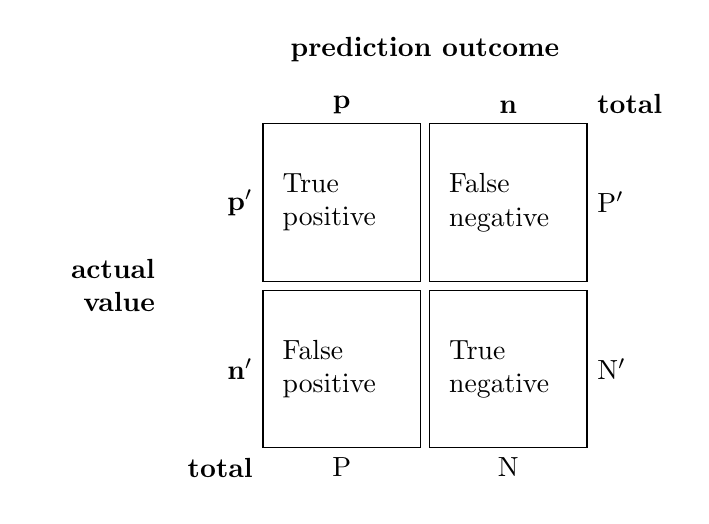
\begin{tikzpicture}[
        box/.style={draw,rectangle,minimum size=2cm,text width=1.5cm,align=left}]
        \matrix (conmat) [row sep=.1cm,column sep=.1cm] {
        \node (tpos) [box,
            label=left:\( \mathbf{p'} \),
            label=above:\( \mathbf{p} \),
            ] {True \\ positive};
        &
        \node (fneg) [box,
            label=above:\textbf{n},
            label=above right:\textbf{total},
            label=right:\( \mathrm{P}' \)] {False \\ negative};
        \\
        \node (fpos) [box,
            label=left:\( \mathbf{n'} \),
            label=below left:\textbf{total},
            label=below:P] {False \\ positive};
        &
        \node (tneg) [box,
            label=right:\( \mathrm{N}' \),
            label=below:N] {True \\ negative};
        \\
        };
        \node [left=.05cm of conmat,text width=1.5cm,align=right] {\textbf{actual \\ value}};
        \node [above=.05cm of conmat] {\textbf{prediction outcome}};
    \end{tikzpicture}
    \caption{Confusion Matrix}
    \label{tab:Confusion Matrix}
\end{figure}



\subsubsection{Receiver Operating Characteristic (ROC):}\hspace*{\fill} \\
Receiver operating characteristics (ROC) (figure~\ref{fig:roc} graphs are useful for organising classifiers and visualising their performance. ROC graphs are commonly used in decision making in machine learning and data mining research. ROC curve provides the False-positive and true positive rates to indicate the performance of the model in different threshold values.~\cite{FAWCETT2006861}

\begin{figure}[H]*
    \centering
    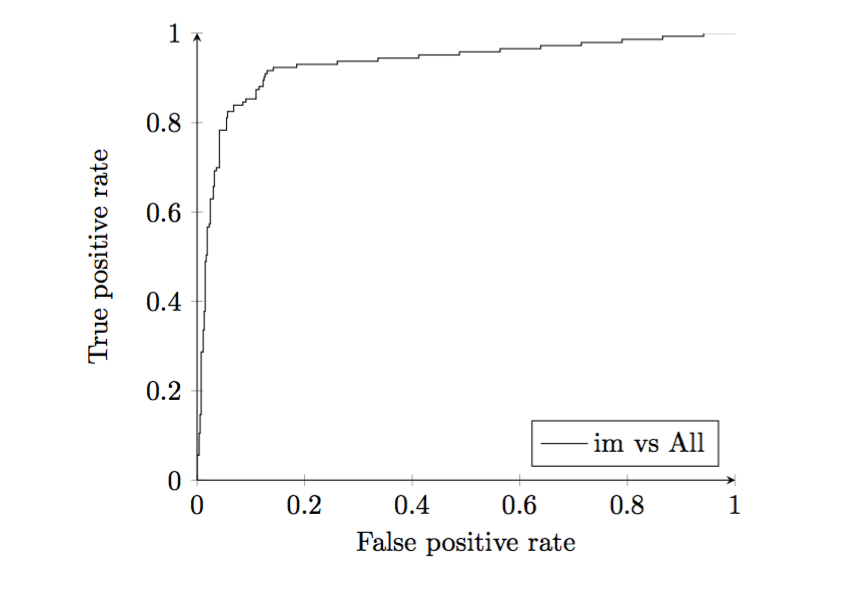
\includegraphics[width=\linewidth]{figures/roc.png}
    \caption{ROC Curve}
    \label{fig:roc}
\end{figure}


\subsubsection{AUC Performance:}\hspace*{\fill} \\
In the case of the imbalanced datasets, not all performance metrics are not suitable. For example, a naive model will provide more than satisfactory accuracy results. Then tool like AUC becomes handy because AUC considers the classification performance by using both positive and negative samples. Hence, AUC can find a reasonable model that classifies imbalanced classes. AUC can be generated by True positive rate (TPR) and false-positive rate. 

\begin{equation} \label{eq:Sensitivity}
    Sensitivity = Recall = \frac{TP}{TP+FN}
\end{equation}

\begin{equation} \label{eq: Specificity}
    Specificity = \frac{TN}{FP+TN}
\end{equation}

AUC is calculated as the Area Under the {Sensitivity` (TPR)- (1-Specificity)(FPR)} Curve.

\section{Design}\label{sec: Design}
Data extracted is a method to gather data for analysing and predicting tasks. Data-driven is a method based on which features can be extracted from the historical data to~\cite{SMARRA20181252}. In classification and prediction problems, it is essential to discover the pattern of the data to get insights. Ensemble learning algorithms and Neural Networks are been found effective~\cite{10.1145/3414274.3414278, RB2021} for real-world pattern detection. This is, however, extremely hard to identify the target information from institutions data and identify patterns to classify the problem. 

The purpose of the chapter is to extract information from a historical dataset and find a suitable classifier for anomaly detection. 



To implement The data-driven machine learning technique that detects suspicious companies to prevent trade-credit fraud, the below system design was used. The design is broadly broken down into main three components. These are Data Mining, Model Configuration, and Model selection. In the below sections each of the components is described. 

\begin{figure}[htp]
    \begin{center} 
    \usetikzlibrary{decorations.text} 
    \newcommand*{\mytextstyle}{\sffamily\Large\bfseries\color{black!85}} 
    \newcommand{\arcarrow}[8]{% 
    % inner radius, middle radius, outer radius, start angle, 
    % end angle, tip protusion angle, options, text 
      \pgfmathsetmacro{\rin}{#1} 
      \pgfmathsetmacro{\rmid}{#2} 
      \pgfmathsetmacro{\rout}{#3} 
      \pgfmathsetmacro{\astart}{#4} 
      \pgfmathsetmacro{\aend}{#5} 
      \pgfmathsetmacro{\atip}{#6} 
      \fill[#7] (\astart+\atip:\rin) arc (\astart+\atip:\aend:\rin) 
           -- (\aend-\atip:\rmid) 
           -- (\aend:\rout) arc (\aend:\astart+\atip:\rout) 
           -- (\astart:\rmid) -- cycle; 
      \path[font = \sffamily, decoration = {text along path, text = {|\mytextstyle|#8}, 
        text align = {align = center}, raise = -.8ex}, decorate] 
        (\astart+\atip:\rmid) arc (\astart+\atip:\aend+\atip:\rmid); 
    } 
    
    \definecolor{grau}{RGB}{208,208,208} 
    \definecolor{mymagenta}{RGB}{226,0,116} 

        \begin{tikzpicture} 
        \fill[even odd rule,mymagenta] circle (2.0); 
        \node at (0,0) (PDCA) {\mytextstyle{\begin{tabular}{c}Development\\Cycle\end{tabular}}}; 
          \arcarrow{3}{3.5}{4}{       0}{    90}{5}{grau,    very thick}{ Data Mining } 
          \arcarrow{3}{3.5}{4}{   180}{   270}{5}{grau,    very thick}{ Feature Engineering } 
          \arcarrow{3}{3.5}{4}{   270}{   360}{5}{grau,     very thick}{ Model Building } 
          \arcarrow{3}{3.5}{4}{     90}{   180}{5}{grau   , very thick}{ Model Evaluation } 
        \end{tikzpicture} 
     \end{center} 
    \caption{Model Development Cycle}
    \label{fig:design}
\end{figure}

\subsection{Data Mining}
The most vital aspect for training a complex system is to feed an adequate dataset, so that model can perform well. However, the information required for preparing a dataset is not readily available in this case.  The steps of data mining techniques are described below. 


\subsubsection{Source Identification}\hspace*{\fill} \\
The subject matter experts are the first point of contact to identify the sources to get the suspicious companies' information. It is important to understand how traditionally the auditors, credit undertaking team analyse the data and identify the key indicators. At the end of the day, fraudulent transaction or activity is human behaviour, hence the experts in this field look for particular patterns and indicators to identify the suspicious entity. The pattern in the financial transaction and general activities of the company are monitored to identify the patterns. Below repetitive steps are taken to identify each key indicator.


\begin{enumerate}
    \item Make a comprehensive list of all possible indicators by taking notes from different subject matter experts. 
    \item Identify if there are any human biases on selected indicators  
    \item Determine if the identified variable is a binary (flag) or continuous variable. 
    \item Identify the source of the data, i.e. internal source (financial statements, company profile) or external source. 
\end{enumerate}


\subsubsection{Data Extraction}\hspace*{\fill} \\
The next activity to prepare the training data set is to extract data from historical company information. Based on the selected key indicators the combined sources are identified. For the current problem, it is been found that the majority of the information is coming from company financial information kept in an Oracle database and historical company reports which are kept in Extensible Markup Language (XML) format. For the data extraction step, all the indicators for the past 10 years have been taken from these sources. The extracted information is kept in the MongoDB server where the information of each company is kept. The financial information is fetched from existing oracle DB, however, the vital company information are extracted from the XML and kept in a JSON format for further uses. 


\subsubsection{Feature Engineering}\hspace*{\fill} \\
After the features extraction feature engineering is done to generate features based on the identified indicators. The engineered features are based on the financial information, company activities and recombination of the information. Due to the sensitivity of the data, the details of the features are not mentioned. However below are the general overview of the feature engineering


\begin{itemize}
    \item \textbf{Financial:} The historical and recent financial information of each company have been collected. This data shows the trend and pattern of the company over the last 10 years. During features extraction, the anomalies are flagged and converted into a binary variable. There are lots of floating points information like yearly profit are kept as a continuous variable. 
    
    \item \textbf{Non-Financial :} The non-financial features are mainly based on the behavioural aspect of personal and the company. As behavioural information is not easily transferable to features, the important activities and characteristics are marked and binary or continuous variables. Information like trade sector, abnormal changes of company, vital dates, recent suspicious transactions etc. are engineered as features.
    
    \item \textbf{Combination:} It was noticed that some of the useful additional features can be mined using the combination method. In a combination method, the new feature can be created combining two or more financial or non-financial features by using logical or mathematical processes. 
\end{itemize}

The pseudo-code structure [Algorithm :\ref{alg:features}] is used to engineer features from extracted data. 

\begin{algorithm}[h]
    \caption{Feature Engineering}
    \label{alg:features}

    \SetKwProg{feature}{Function \emph{feature}}{}{end}
    
        \feature{(Company Object)}{
            \textbf{Input:}{ company information in JSON formal} \\
            \textbf{Output:}{ feature value (int - flag, float for continues variable}
      
            \State {$feature\_counter \gets 0$ \CommentSty{Initialise the counter}} \\
            
            \If{ $report\_date$ is available}{
                  $important\_date$ = $report\_date$\;
              }
            \Else{}{\Return $feature\_counter$}
             
            \State {$json\_expression$ \= parse JSON to get feature information} \\
            \State{$list \gets$ value from $json\_expression$ }\\
           \\
            \ForAll{child $c$ in list}{
                \If{$important\_date \leq child['date']$ }{
                        $feature\_counter$ ++
                    }
                 
            }
            \Return $feature\_counter$\\
        }

\end{algorithm}




\subsection{Model configuration}

\subsubsection{Random Forest}\hspace*{\fill} \\
Random forest algorithm generally performs better compare with other classification algorithms for imbalanced dataset \cite{Valecha2018PredictionOC}. In random forest model classifier ensemble different trees and final prediction happens by voting and selecting the majority decision. 

\begin{enumerate}
    \item Randomly select N number of Features
    \item Train a Decision Tree with selected features
    \item Select the target number of tress and repeat first two steps 
    \item Each tree predicts the class for new entry
    \item The final class prediction done by majority vote. 
\end{enumerate}

\textbf{Hyper-parameter tuning:}
Random Forest classifiers come with crucial parameters which need to be tuned to get the best model. Below parameters are used in a random grid search method to do hyperparameter tuning for the random forest estimator. The options for each estimator are shown in the table: ~\ref{tab:RF_param}.

\begin{itemize}
    \item n\_estimator: Number of trees in random forest
    \item max\_features: Number of features to consider at every split
    \item max\_depth: Maximum number of levels in a tree
    \item min\_samples\_split: Minimum number of samples required to split a node
    \item min\_sample\_leaf: Minimum number of samples required at each leaf node
    \item bootstrap: Method of selecting samples for training each tree
\end{itemize}

\begin{table}[h]
    \begin{tabular}{llll}
    Parameter           & Options         & No of options \\
    n\_estimator        & 200 to 2000     & 100           \\
    max\_features       & Auto, sqrt      & 2             \\
    max\_depth          & None, 10 to 110 & 12            \\
    min\_samples\_split & 2,5,10          & 3              \\
    min\_samples\_leaf  & 1,2,4           & 3              \\
    bootstrap           & True, False     & 2              \\
    \end{tabular}
    \caption{Hyper-parameter settings for Random Forest}
    \label{tab:RF_param}
\end{table}


\subsubsection{XGBoost}\hspace*{\fill} \\
Tree boosting is also effective ensemble learning learning method~\cite{2016}. XGBoost is used widely by data scientists to achieve state-of-the-art results on many machine learning challenges.To apply XGBoost model we have use below parameters. 

By n\_estimator parameter can be selected based on the performance of the initial run. To optimize max\_depth parameter the depth search started from 3 to 10 by gradually increasing. To avoid overfitting learning rate parameter comes in handy for the XGBoost Algorithm. The subsample is for each tree percentage of rows are taken to build the tree. The colsample\_bytree is used by each tree to select the proportion of the column. Below are the details of the parameter tuning for XGBoost. 

\begin{itemize}
    \item learning\_rate: 0.01
    \item n\_estimators: 100 to 1000 range 
    \item max\_depth: 3 to 10 
    \item subsample: 05. to 0.8
    \item colsample\_bytree: 1
    \item gamma: 1 
\end{itemize}

\subsubsection{Artificial Neural Network (ANN)}\hspace*{\fill} \\
The configuration of neural networks is of of the toughest part of applying neural networks. There are different types of neural networks are available for classification problems. Considering the existing dataset a fully connected 10 layers neural network is used. Below is the configuration of the neural network built for the given tasks.  

\begin{table}[] 
\begin{tabular}{lll} 
Model: Model\_1 \\ \hline 
 Layer (type)                  & Output Shape                & Param \#    \\ \hline \hline 
 dense (Dense)                 & (None, 27)                  & 756        \\ \hline 
 dense\_1 (Dense)               & (None, 15)                  & 420        \\ \hline 
 dense\_2 (Dense)               & (None, 1)                   & 16         \\ \hline 
===============================& ============================& ===========\\ \hline \hline 
Total params: 1,192 \\ 
Trainable params: 1,192 \\ 
Non-trainable params: 0 \\ \hline 
\end{tabular} 
\caption{Model summary for Model\_1.} 
\label{tab:model-summary} 
\end{table}

After trying with different shapes and sizes of the network, it was found that 10 layers work the best for the given dataset. Relu activation functions are used in the dense and sigmoid aviation for the output layer are used. To overfitting, the model dropout parameter is used, however, it is been found that L1 and L2 regulators do not perform well in this scenario. 



\section{Evaluation}\label{sec: Evaluation}
%Discuss the design of your experiments, the results you obtained,and how they help in evaluating the claims you made in the introduction. You may also use the evaluation results in this section to justify your design choices or assess the contributions of different aspects of your design towards the overall goals.

The result section of the report is divided into two parts. In the first part, the outcome of the data mining is shown under the section exploratory data analysis. In the second section performance of the models are noted down. 

\subsection{Exploratory data analysis}

\subsubsection{Dataset}\hspace*{\fill} \\
The data extraction method mentioned in the section~\ref{sec: Design} was followed to generate the dataset from the historical company information.

To prepare this dataset, the historical data from 2011 to 2021 is considered. During the considered period, a company would generally have multiple status reports, however, to get the latest updates of each company the last report was considered. The reports are also filtered out based on the report type as not all reports would have all the required information. 

The data extraction and feature engineering processes are very time-consuming. To make sure these processes run within an acceptable time and to support our design method, 25\% majority classes were not included while preparing the dataset. From the paper on SMOTE~\cite{2002}, we have seen the under-sampling with SMOTE performs relatively well. So theoretically the performance will still get improvement.

In the generated dataset, there are a total of 30 columns available. Out of which three columns are report date, report id, these three columns were dropped before the training. However, these columns are used for identifying the company information after the training. 

 27 columns were selected as the features, the remaining one column contains the class information, which was used for the training label.  

The total number of instances is 48,549. Among this data, only 1358 are marked suspicious companies. As mentioned earlier the actual data was filtered to avoid duplicated and inadequate reports. 
\begin{itemize}
    \item Total number of columns: 30
    \item Number of company entries: 48,539
    \item Target label: Suspicious
    \item Total Features: 27
    \item Total suspicious cases: 1358
\end{itemize}


\subsubsection{Class Distribution}\hspace*{\fill} \\
From the initial assessment we can see the that classes are very imbalanced. In the dataset there is only 1358 fraudulent cases out of 48,549 ones. That means only 2.8\% of companies are fraudulent or specious [shown in figure~\ref{fig:class distribution}]. However as mentioned in the dataset section above, 25\% of majority class were under samples during the dataset preparation. That means the actual class distribution is much lower in reality. However to make a realistic model, we will consider this class distribution in the rest of the paper. 

\begin{figure}[H]
    \centering
    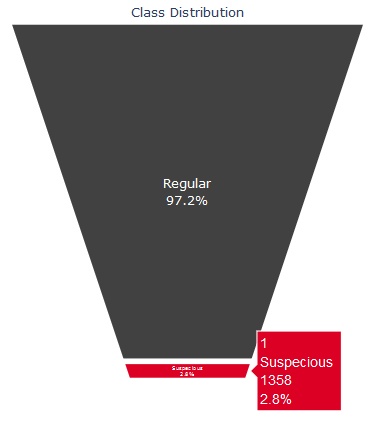
\includegraphics[width=.8\linewidth]{figures/class_imbalance.png}
    \caption{Class Distribution}
    \label{fig:class distribution}
\end{figure}

Even after the undersampling of the majority class, we can see from figure~\ref{fig:class distribution} that our dataset is highly imbalanced. Hence during the training of different models, we had to try different sampling methods to feed the model with a similar class distribution. In the model performance section with and without SMOTE is shown. 

\subsubsection{Task complexity}\hspace*{\fill} \\
From the class distribution, we can already assume that classifying suspicious classes would be extremely hard. To understand the complexity more, dimension reduction functions were applied to visualize the class distribution in a two-dimensional space. As we can find the figure~\ref{fig:Dimension reduction}, the classes cannot be easily separated. So the classes are not only imbalanced but also closely related. That means complexity to build a model to detect suspicious class would be a huge challenge.
 
\begin{figure}[H]
    \centering
    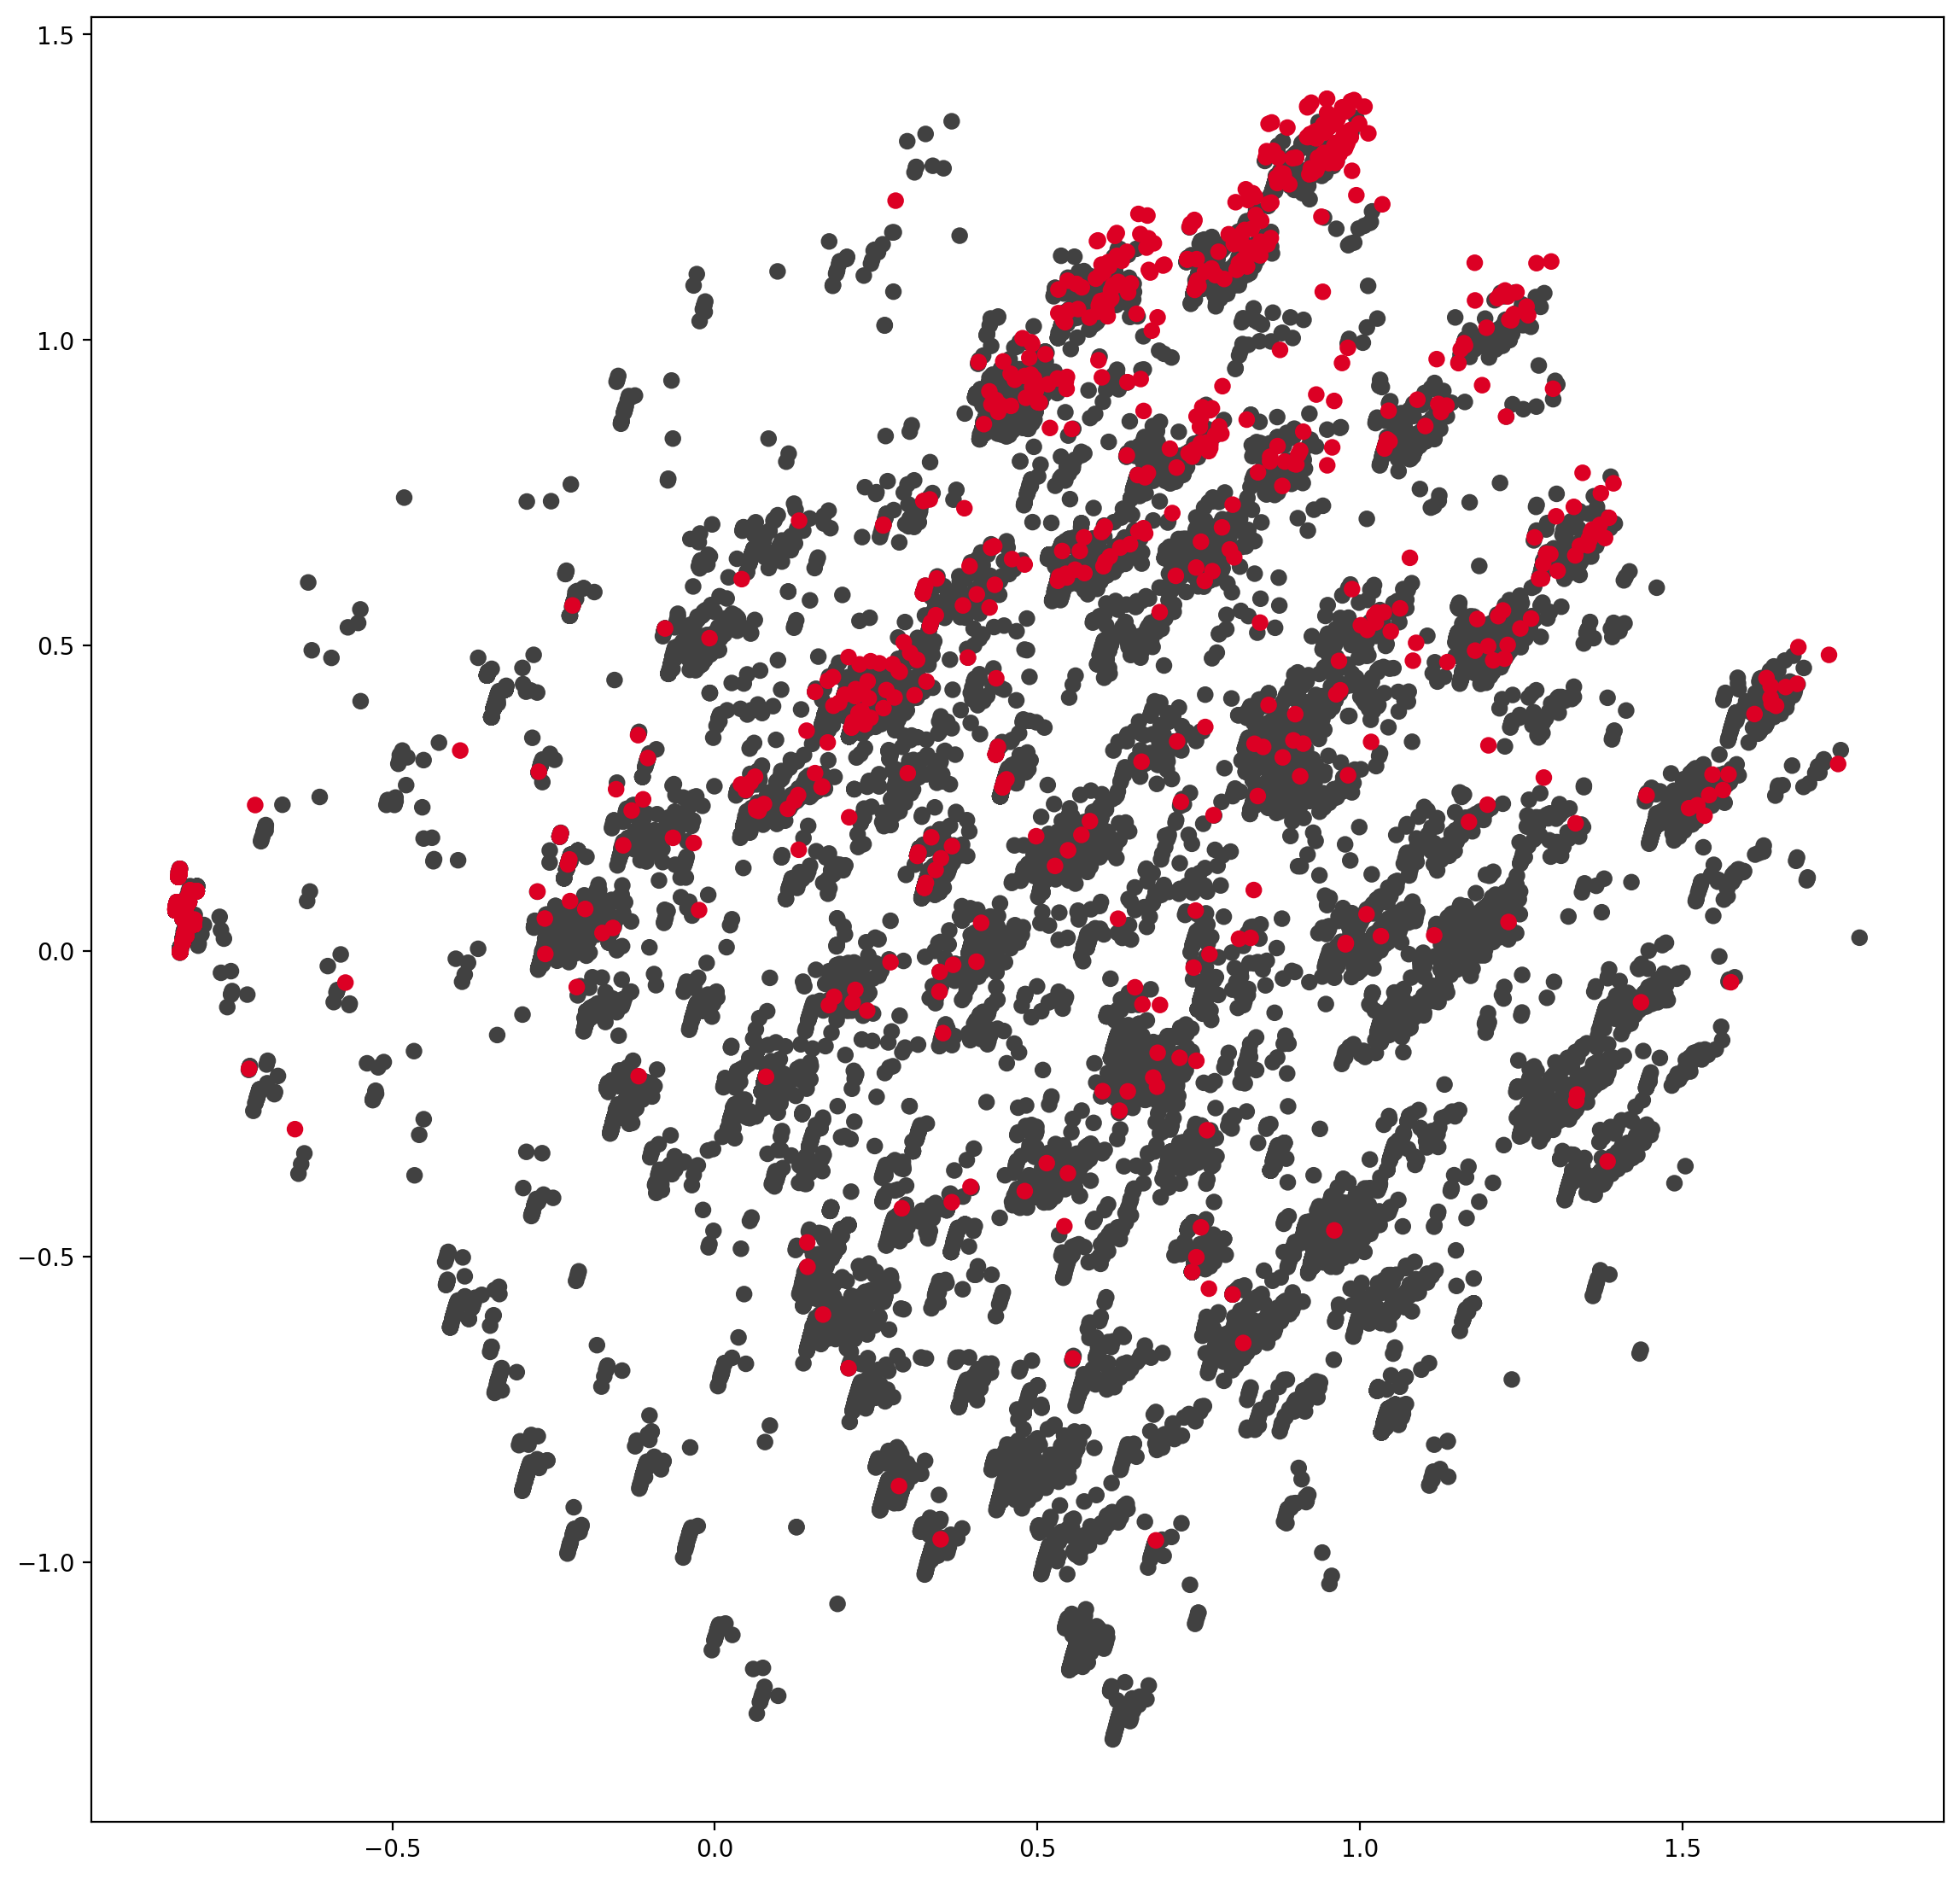
\includegraphics[width=\linewidth]{figures/pca_2d.png}
    \caption{Classes after Dimension reduction}
    \label{fig:Dimension reduction}
\end{figure}


\subsubsection{Class Proportion}\hspace*{\fill} \\
 It is important to understand the effectiveness of the selected features. Theoretically, we want to select the features which have the indication of suspicious patterns. To do so, the proportion of the classes based on features were prepared. In the figure~\ref{fig:feature proportion} the proportion of the binary features are shown.
\begin{figure}[H]
    \centering
    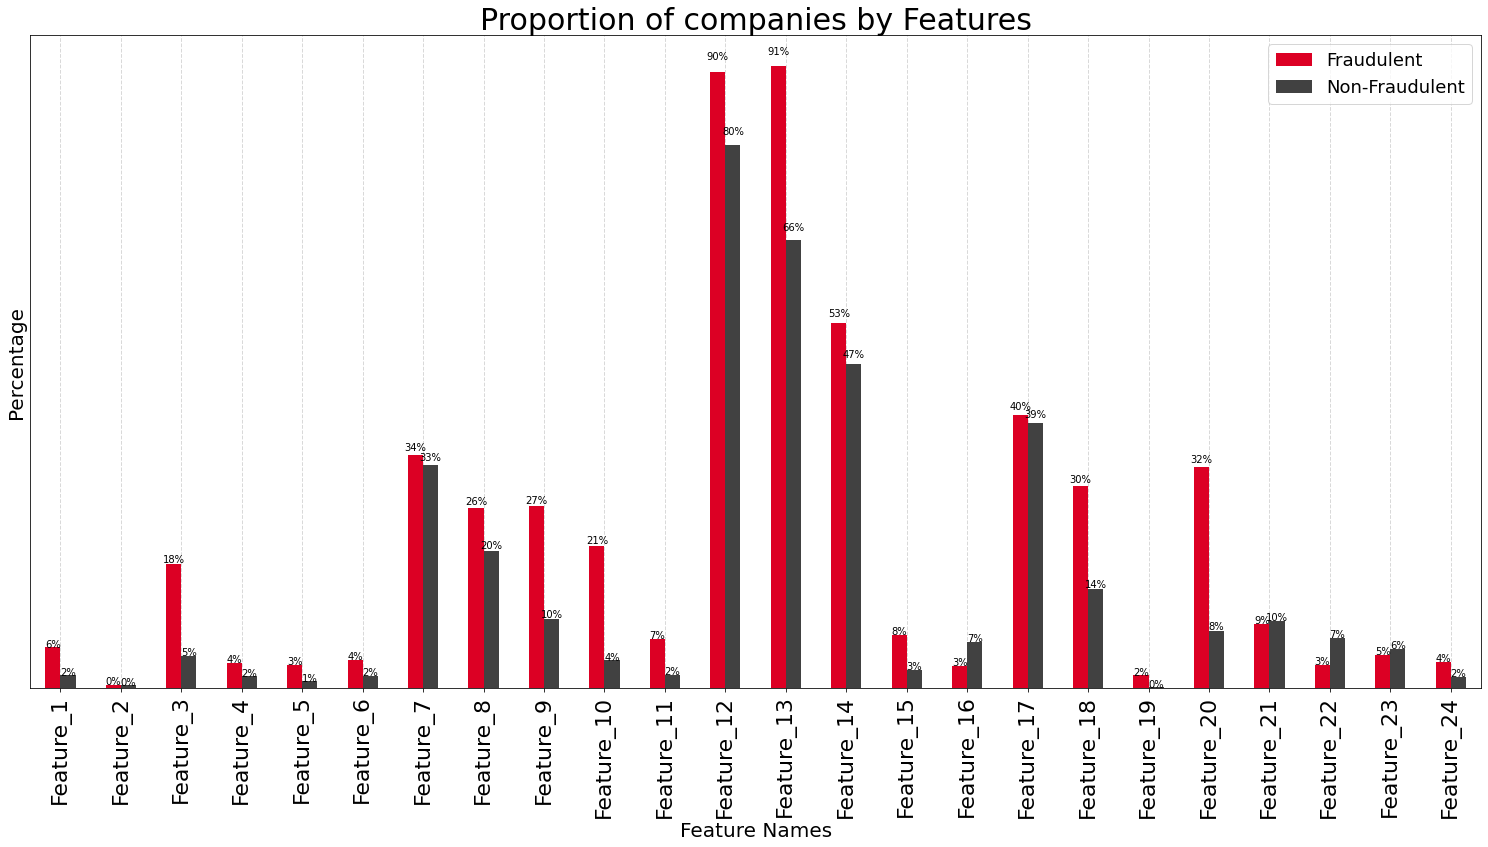
\includegraphics[width=\linewidth]{figures/feature_proportion.png}
    \caption{Proportion of binary features}
    \label{fig:feature proportion}
\end{figure}

From the figure~\ref{fig:feature proportion} we can see that majority of the engineered features has a higher proportion of suspicious classes than regular classes. This is a good indication that the selected features may help the model classify the patterns. 


For the continues variable statistical information like mean, median and standard deviation between two classes were considered to find the effectiveness of the features. The figure~\ref{fig:Continues Feature Statistics} shows the statistics of the continues variable features. 

\begin{figure}[H]
    \centering
    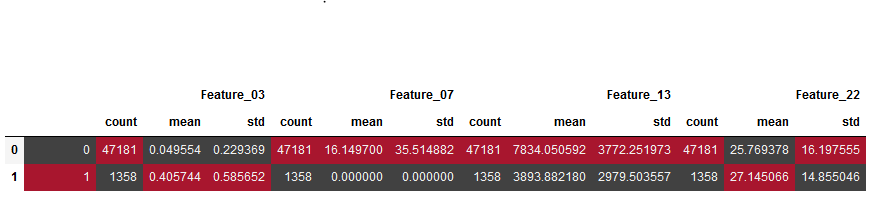
\includegraphics[width=\linewidth]{figures/feature_proportion_2.PNG}
    \caption{Continues Feature Statistics}
    \label{fig:Continues Feature Statistics}
\end{figure}


\subsubsection{Correlation Matrix}\hspace*{\fill} \\
A good visualization tool to understand the relation between classes and features is the correlation matrix. In figure~\ref{fig:corr} we can visualize the relation between suspicious class and respective features. At a glance, we can see that the correlation between features and classes are very low. That is a good reference to understand the complexity of the tasks. 
\begin{figure}[H]
    \centering
    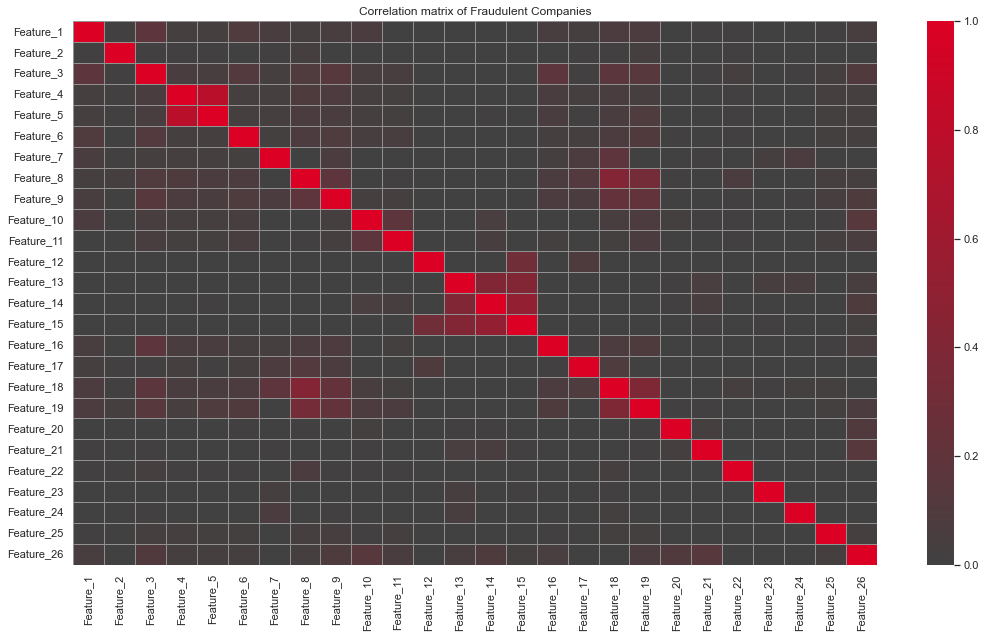
\includegraphics[width=\linewidth]{figures/corr.png}
    \caption{Correlation Matrix}
    \label{fig:corr}
\end{figure}

\subsection{Model Performance Results}\label{sec: model results}

To select the right classifier, it is important to verify the performance of each model by using all types of performance matrices. For this paper to select we will use the mentioned method in the section Tools of trades in the Design Overview section. The below subsections provide the performance of each model in different matrices. 


There is a total of six models we have selected for comparison. We have random foreset, XGBoost, and artificial neural networks models and their variation with SMOTE. 

\subsubsection{Performance Metrics:}\hspace*{\fill} \\
In the table~\ref{tab:per_res} the performance results of Random Forest, XGBoost, and Artificial Natural networks are shown. Each model has with and without SMOTE version. Each models performance results are shown in the respective rows. The columns show, accuracy, precision, recall and f1-score for each respective model over the test dataset. 
\begin{table}[H]
    \begin{tabular}{clrrrr}
    \cline{1-6}
    \multicolumn{1}{l}{SMOTE} & Model         & \multicolumn{1}{l}{Accuracy} & \multicolumn{1}{l}{Precision} & \multicolumn{1}{l}{Recall} & F1 \\ \cline{1-6} 
    \multirow{3}{*}{No}       & Random Forest &0.97  & 0.42  & 0.07  & 0.11 \\
                              & XGBoost       &0.97  & 0.44  & 0.03  & 0.06 \\
                              & ANN           &0.97  & 0.30  & 0.10  & 0.15 \\ \cline{1-6} 
    \multirow{3}{*}{Yes}       & Random Forest &0.88  & 0.11  & 0.47  & 0.17 \\
                              & XGBoost       &0.88  & 0.10  & 0.47  & 0.17 \\
                              & ANN           &0.86  & 0.09  & 0.46  & 0.15 \\ \cline{1-6} 
    \end{tabular}
    \caption{Test Data performance}
    \label{tab:per_res}
\end{table}


The figure~\ref{fig:test_train} shows the performance results of each model in bar charts. The columns show the f1-performance results of each model. The bars are clustered into performance results of train and test datasets. 

\begin{figure}[H]
    \centering
    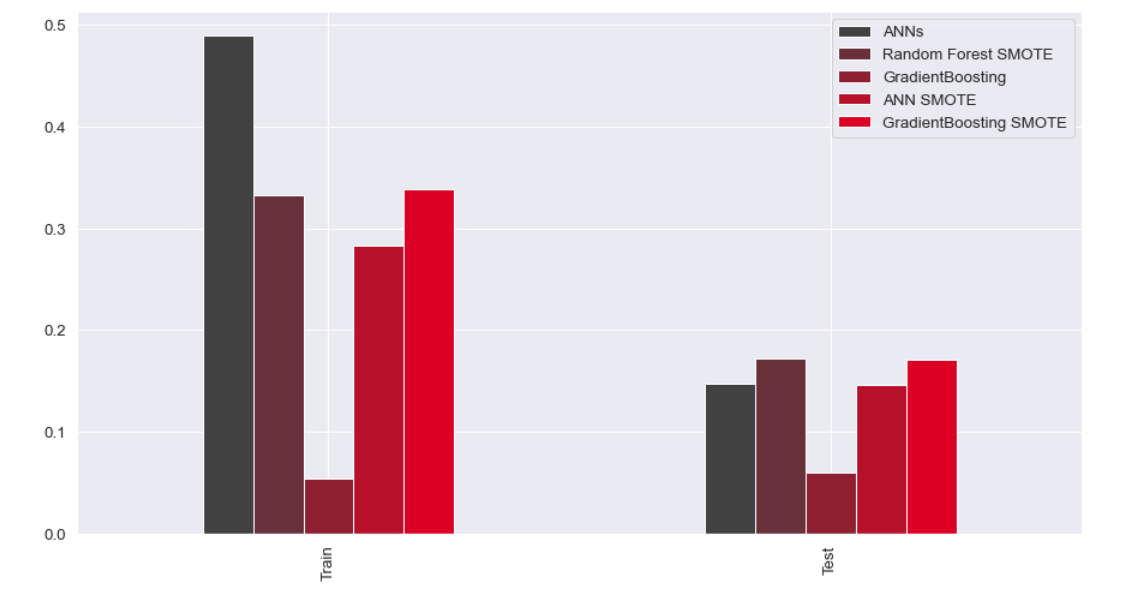
\includegraphics[width=\linewidth]{figures/results.PNG}
    \caption{Performance over train and test data}
    \label{fig:test_train}
\end{figure}

\subsubsection{ROC curve}\hspace*{\fill} \\
Figure~\ref {fig:roc_all} shows the ORC curves of all the models in a single place. The x-axis indicates the false positive rate, and the y-axis indicates the true positive rate. The ROC curves are placed together in this figure for visual comparison. 
\begin{figure}[h]
    \centering
    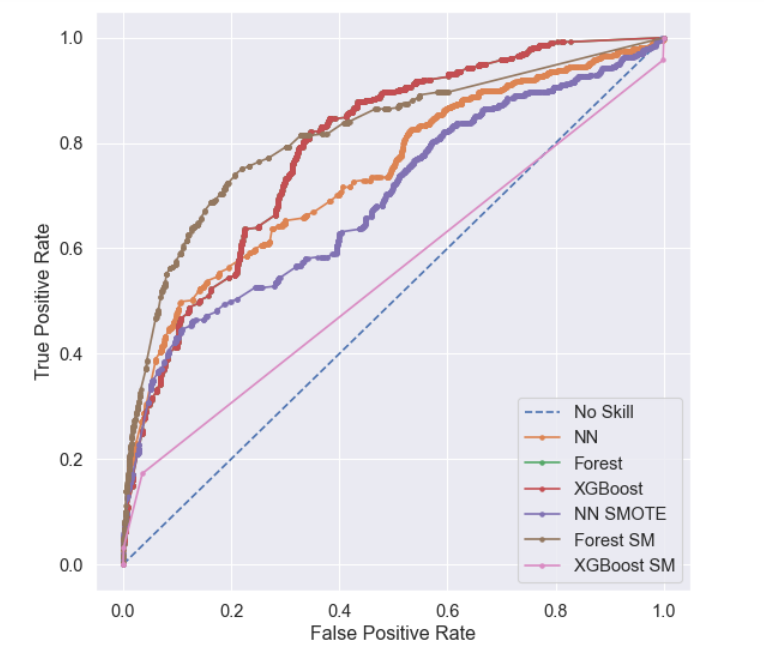
\includegraphics[width=\linewidth]{figures/roc_res.PNG}
    \caption{ROC Curves}
    \label{fig:roc_all}
\end{figure}

In the figure~\ref{fig:roc_all_2} ROC curves are displayed in comparison with no skill classifiers. This gives a visual demonstration of the area under the curve. 
\begin{figure}[h]
    \centering
    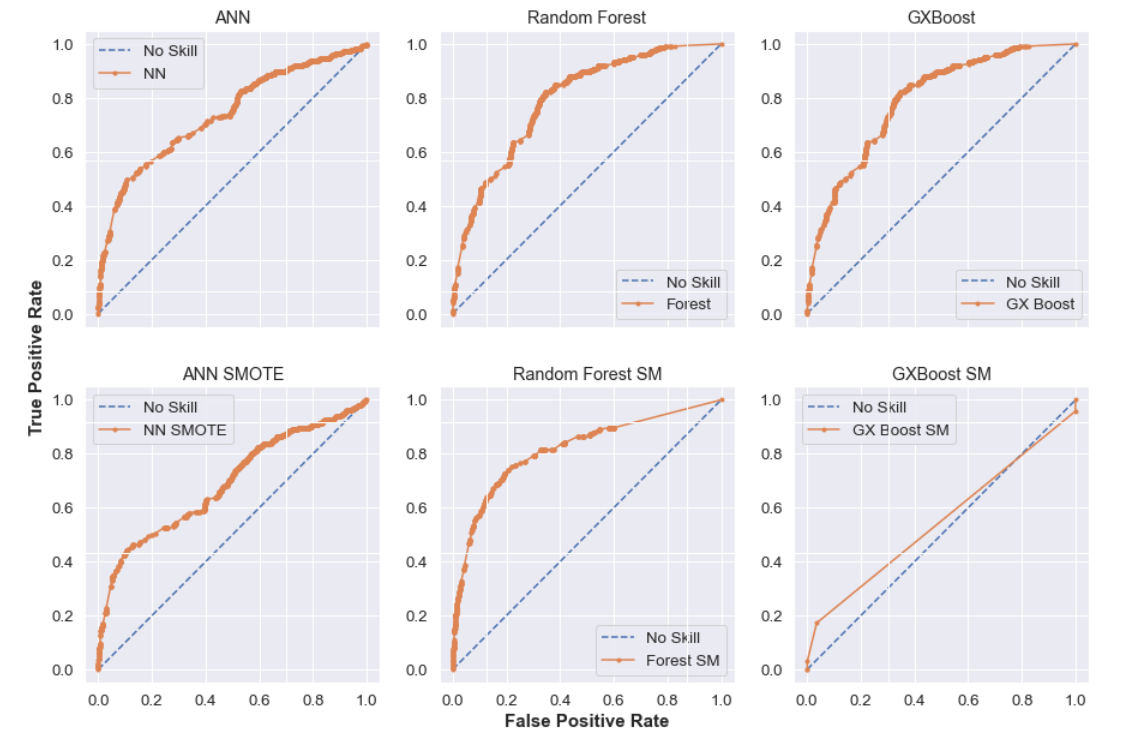
\includegraphics[width=\linewidth]{figures/roc_res_full.PNG}
    \caption{ROC Curves compare to no skill model}
    \label{fig:roc_all_2}
\end{figure}


% \mytodo{model selection hint\: %https://medium.com/@matteding/imbalanced-data-fraud-detection-3185c1cdaa77}

\subsubsection{AUC ROC}\hspace*{\fill} \\
AUC ROC Curve means the area under the ROC curve. The AUC ROC values for each model is shown in the table~\ref{tab: roc_auc}. The values help us to choose the best model when it's difficult to see from the ROC curve visually. 
\begin{table}[H]
    \begin{tabular}{|l|l|}
    \hline
    MODEL     & ROC AUC \\ \hline
    No Skill  & 0.500   \\ \hline
    ANN       & 0.742   \\ \hline
    RF        & 0.793   \\ \hline
    XG        & 0.725   \\ \hline
    ANN SMOTE & 0.693   \\ \hline
    RF SMOTE  & 0.817   \\ \hline
    XG SMOTE  & 0.549   \\ \hline
    \end{tabular}
    \caption{ROC AUC Values}
    \label{tab: roc_auc}
\end{table}


\subsubsection{Confusion Matrix}\hspace*{\fill} \\
In the figure~\ref{fig:cm_rf} the performance of the random forest with SMOTE is shown in a form of a confusion matrix. In the matrix predicted labels and trues labels are shown in a 2 by 2 matrix. The bottom right box shows the True positive cases on the other the top right shows the false-positive results on the test data. 
\begin{figure}[H]
    \centering
    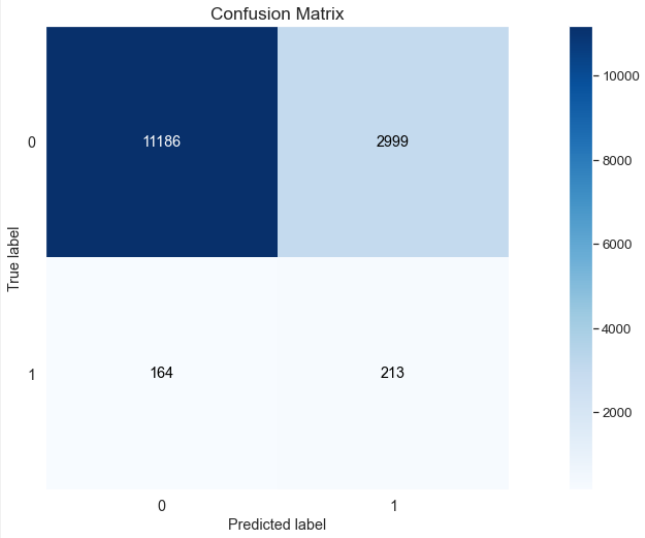
\includegraphics[width=\linewidth]{figures/cm.PNG}
    \caption{Confusion Matrix Random Forest}
    \label{fig:cm_rf}
\end{figure}


\subsubsection{Threshold value}\hspace*{\fill} \\
To verify the performance of the model is also important to see how the performance of the model works in the different thresholds. Figure~\ref{fig:cm_r} shows all the values of the random forest model. The thresholds values chosen for the model are 0.1, 0.15, 0.2, 0.25, 0.35, 0.4, 0.45 and 0.5. 
\section{Discussion}\label{sec: discussion}
In this section, the discussion on the results presented in section~\ref{sec: Evaluation} is covered. The main discussion focuses on the performance comparison of each model. Based on section~\ref{sec: model results} of this report, the result discussion is covered. 

\subsubsection{Performance Metrics}\hspace*{\fill} \\
It is apparent from this table~\ref{tab:per_res} that accuracy for the models is not a suitable matrix. All the non SMOTE models got 97\% accuracy and for SMOTE models the accuracy varies from 86\% to 88\%. Considering the huge class imbalance we know even a naive model will give around 98\% accuracy. 

The results of precision metrics drop significantly from non-SMOTE to SMOTE models. In SMOTE models XGBoost has the highest precision rate of 0.44 and the artificial neural network has the lost rate of 0.30. For SMOTE group, the Random Forest model has the heights precision value of 0.11, which is significantly lower than the values in the no Smote group.   

The recall is a good matrix for imbalanced data set like this. In the table~\ref{tab:per_res} we can see that the recall performance of the models' increases from SMOTE than non SMOTE group. Random Forest and XGBoost with SMOTE have a heights recall score of 0.47. 

We see the f-1 score remain unchained for the artificial neural network. The f1-score improves significantly for XGBoost from 0.06 to 0.17 after SMOTE transformation. Random Forst with SMOTE also has a heights score of 0.17 which increase by .6 points. 


In the figure~\ref{fig:test_train} we can see that as expected the performances of all the model drops from train set to test set. The random forest model has the highest value (more than 0.8) in the train set, however, the performance dramatically drops for the test data. Similarly, ANN performs well in the train set however the performance test drops but not as much as random forest. The XGBoost performs the worst in both train and test data. From this chart, we can see the XGBoost and Random Forest with SMOTE performs well in the test dataset. 


\subsubsection{ROC Curves}\hspace*{\fill} \\
The results of the ROC curves are shown in figure~\ref{fig:roc_all}and in figure~\ref{fig:roc_all_2}. ROC curves give the idea of how the model performs for True Positive (TF) and False Positive (FP) cases. The no skill line shows us the guideline for the comparison of the models. From the figures, we can see that Random Forest with SMOTE appears to have the best ROC curve. On the other hand, XGBoost which looked promising in the table ~\ref{tab:per_res} completely fails the ROC curve tests. We can see the results gradually increases till 0.2, however, then it hardly performs any better than no skill models. The rest of the models perform similar to each other. 


\subsubsection{AUC ROC}\hspace*{\fill} \\
From the ROC curve analysis, we already got the Idea that the Random Forest with SMOTE performs the best. However, besides the XGBoost with SMOTE, most of the models' performance looks similar. The rest of the models' seems to have a similar area like Random Forest, hence checking the area under the curve by AUC ROC metrics is a good way for this scenario. In table~\ref{tab: roc_auc} we can see that Random Forest with SMOTE has the highest ROC AUC score of 0.817. XGBoost with SMOTE has the lowest 0.549 which is just a little better than the no skill model. The rest of the models as found in the ROC analysis have similar ROC AUC values starting from 0.693 to 0.793.


After analysing all the matrices we can say that the Random Forest with SMOTE performs the best among all the models. However, the overall performance of all the models is quite low. In the confusion matrix for our best model Random Forest with SMOTE, in the figure~\ref{fig:cm_rf}, we can see that only 213 suspicious cases were properly classified. The model fails to detect 164 cases and also gives a high false-positive case of 2999. After changing the threshold values, figure~\ref{fig:cm_rf_full} we can see that models tend to perform better, however, after the 0.4 threshold value, the models get a huge number of false positives. This is a clear indication that there is a scope of improvements. 
\section{Conclusion}\label{sec: conclusion}
% inital part of the conclusion



% additional points
Trade fraud is not only causes Economic damage to the business and their respective financial institutions, but also creates disrupt in the overall economy. Sometimes fraudulent companies use the fund for terrorism, human rights violation, money laundering.
\section{Future Work}\label{sec:future-work}

\begin{itemize}
    \item Deep sampling method can be applied 
    \item Genetic algorithm 
    \item Other types of neural networks like CNN, transformers 
\end{itemize}


\newpage
\appendix
\section{Appendix}\label{sec:appendix}
\lipsum[2-3]


\newpage
\addcontentsline{toc}{section}{References}
% \bibliographystyle{ACM-Reference-Format}
% \bibliography{ref.bib}
% \addbibresource{}
\printbibliography

\end{document}
